\documentclass[../main.tex]{subfiles}

\begin{document}
\cleartooddpage[\thispagestyle{empty}]
\phantomsection\addcontentsline{toc}{part}{Appendices}
\originalpart*{Appendices}

% \chapter{Material}
% Here follows a brief description of the material used in this thesis
% \section{Hardware}
% A portable personal computer
% \begin{description}
% \item [Processor] Intel(R) Core(TM) i7-8750H CPU @ 2.20GHz
% \item [Memory] 15GiB System memory
% \end{description}
% \section{OS}
% A GNU/Linux system based on architecture x86\_64 with
% \begin{description}
%     \item[Linux kernel] version 5.4.0-73-generic
%     \item[Ubuntu distribution] version \#82~18.04.1-Ubuntu SMP Fri Apr 16 15:10:02 UTC 2021
% \end{description}

% \section{Programming}
% The programs used in this thesis were developed in MATLAB language.

% They were executed on
% \begin{description}
% \item[MATLAB] version R2019b Update 3 (9.7.0.1261785) 64-bit (glnxa64).
% \end{description}

% All code and resulting data is available in \todo{add github link}.

% The graphs based on the saved data were generated using python scripts, also available.

% The scripts were then executed using
% \begin{description}
% \item[python] version 3.6.9
% \end{description}
% with packages:
% \begin{description}
%     \item[matplotlib] version 3.2.2
%     \item[numpy] version 1.19.0
%     \item[scipy] version 1.3.2
% \end{description}
% \section{Writing}
% This thesis was written using GNU Emacs, typeset using \gls{latex}.

% Diagrams were drawn using \gls{TikZ}.

% Hand drawings were drawn using Xournal++ and Inkscape.

\chapter{Résumé étendu en français}

\section{Contexte et Motivation}\label{sec:cont-et-motiv}

Pour illustrer on donne un example, ou
\begin{figure}[H]
  \centering
  \begin{tikzpicture}[font=\small,thick,node distance=3*0.6180cm and 0.6180cm,every node/.style=rectangle,
    mpcSmall/.style={fill=mpc_agent, minimum height=0.6180*2cm, minimum width=2cm},
    coordinator/.style={fill=mpc_coordinator, minimum height=0.6180*3cm, minimum width=6cm},
    ]

    \node[draw, mpcSmall,] (block1) {\small Maison 1};
    \node[fill=none, draw=none, right=of block1,] (mult) {\bf $\dots$};
    \node[draw, mpcSmall, fill=mpc_agent, right=of mult,] (blockM) {\small Maison M};
    \node[draw, coordinator, below=of mult,] (coordinator) {Coordinateur};

    \draw[-latex,line width=1pt] (block1.south)+(0.4,.0) -- ( coordinator.north -| {$(block1.south)+(0.4,.0)$}) node [right,midway] {$\lambda_{1}$};
    \draw[latex-,line width=1pt] (block1.south)+(-0.4,0) -- (  coordinator.north -| {$(block1.south)+(-0.4,0)$}) node [left,midway] {$\theta_{1}$};
    \draw[-latex,line width=1pt] (blockM.south)+(0.4,.0) -- ( coordinator.north -| {$(blockM.south)+(0.4,.0)$}) node [right,midway] {$\lambda_{M}$};
    \draw[latex-,line width=1pt] (blockM.south)+(-0.4,0) -- (  coordinator.north -| {$(blockM.south)+(-0.4,0)$}) node [left,midway] {$\theta_{M}$};
  \end{tikzpicture}
  \caption{Échange entre contrôleurs locaux et coordinateur.}\label{fig:echange_controleurs_coordinateur}
\end{figure}
\begin{quote}
  \raggedright
  Les allocations $\theta_{i}$ sont proposées pour chaque maison par le coordinateur.
  Le contrôleurs locaux respondent avec des indices $\lambda_{i}$ qui indiquent leur satisfaction.
  Les allocations sont mises à jour basées sur ces indices jusq'un consensus soit établi.
\end{quote}

\begin{figure}[H]
  \centering
  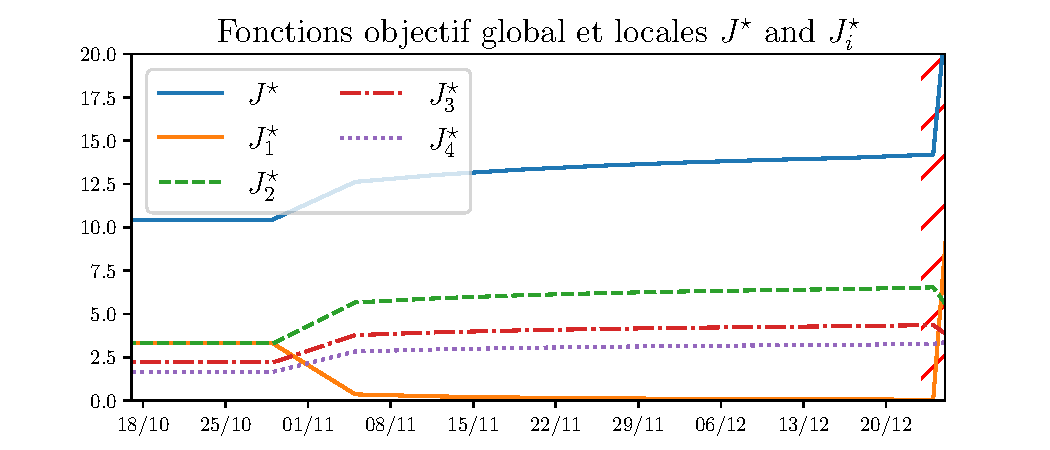
\includegraphics[width=.8\textwidth]{../img/example_introduction/example_J_fr.pdf}
  % ./docstheseplot -o ../../docs/img/quantiteAvecTriche4 -i  ../../data/matlab/tricheQuantite/dmpcQuantity4systemsTriche_.mat --quantiteAvecTriche4
  \caption{Graphique des fonctions objectives dans une période de 10 semaines.}\label{fig:change_in_j}
\end{figure}
\simplebox{
  \begin{itemize} \bfseries
    \item Peut-on detecter l'attaque?
    \item Peut-on identifier l'attaqueur?
    \item Peut-ont miniser les effets du dit attaque?
  \end{itemize}
}
Cette thèse a comme objectif répondre ces questions dans un cas spécifique qui sera formalement presenté.
Pour mieux comprendre et répondre ces questions, on divise ce travail en deux parties:

\paragraph{La première partie} (\S~\ref{sec:comm-pred-et} à~\ref{sec:comp-anorm}) sert comme une gentille introduction au déssin des \dmpc{}, à sa sécurité et à des attaques.
\newcommand{\tpc}{\textperiodcentered}

Pour un\tpc{}e lecteur\tpc{}ice pas familiarisé\tpc{}e, Section~\ref{sec:comm-pred-et} explique ce qui est une Commande Prédictive et les défis pour la décomposer.
Section~\ref{sec:differents-topologies} discute les topologies possibles pour fair la décomposition.
Section~\ref{sec:comp-anorm} définit comportements anormaux, donne quelques examples, les catégorise et présente les méthodes pour les prévenir et combattre.

\paragraph{La seconde partie} (\S~\ref{sec:vulnerabilites-de-la} à~\ref{sec:comm-pred-resil-1}) contient les contributions de cette thèse.

Section~\ref{sec:vulnerabilites-de-la} présente la décomposition étudié (décomposition primal). On presents ses vulnérabilités et comment elles peuvent affecter la perfomance du système.
On formalise l'example en donnant une approche plus quantitative.
Une fois les vulnérabilités et les possibles effets des attaques découverts, on divise la mitigation en parties plus gérable.
\\ Premièrement en Section~\ref{sec:comm-pred-resil}, on analyse un problème simple, pour qu'on puisse apprécier les possibles difficultés qui peuvent être rencontrées pendant le problème de mitigation.
À partir de cette analyse, on propose des mécanismes de detection et mitigation, suivis par un example académique pour illustrer leur fonctionnement.

\\Après, en Section~\ref{sec:comm-pred-resil-1}, on analyse un problème similaire mais avec un coup de théâtre. Comme on verra, une petite modification du problème inital cause une augmentation exponentiel de sa complexité.
L'analyse de ce nouvel problème résulte une stratégie similaire, mais avec modifications adéquates pour renfermer la nature exponentiel du problème.

Finallement, on conclue le travail avec Section~\ref{sec:conclusion_resume}, où on discute les résultats de l'étude, ses bénéfices et inconvénients.
La discussion ouvre des questions qui peuvent inciter des nouveau travaux.

\newpage
\section{Commande Prédictive et sa décomposition}\label{sec:comm-pred-et}

\newpage
\section{Differents topologies}\label{sec:differents-topologies}

\newpage
\section{Comportements anormaux}\label{sec:comp-anorm}

\newpage
\section{Vulnerabilités de la decomposition primal}\label{sec:vulnerabilites-de-la}

\newpage
\section{Commande Prédictive résiliente pour systèmes dépourvus}\label{sec:comm-pred-resil}
\newpage
\section{Commande Prédictive résiliente sur pénurie artificielle}\label{sec:comm-pred-resil-1}

\newpage
\section{Conclusion}\label{sec:conclusion_resume}
\end{document}
